\documentclass{beamer}
\usepackage[utf8]{inputenc}
\usepackage{hyperref}
\usepackage{multicol}
\usepackage{hyperref}
\usepackage{verbatim}

\inputencoding{utf8}

\mode<presentation> {
    \usetheme{Madrid}
}

\usepackage{graphicx}
\usepackage{booktabs}

\title[Git]{Control de versiones y Git}
\author{Ernesto Rodriguez}
\institute{
    Universidad del Itsmo \\
    \medskip \textit{erodriguez@unis.edu.gt}
}

\date[\today]{}

\begin{document}

\begin{frame}
\titlepage
\end{frame}

\begin{frame}
\frametitle{Control de versiones}
\begin{itemize}
    \item{El proceso de llevar un registro de todos los cambios que 
    han habido en un repositorio.}
    \item{Un {\emph repositorio} es un conjunto de archivos y recursos
    que confrman algun proyecto. Generalmente, un proyecto de software.}
    \item{El contenido de un repositorio se representa mediante revisiones.}
    \item{Un \emph{controlador de versiones} es una herramienta que permite
    llevar el control de versiones.}
    \item{Existen varios controladores de versiones: Git, Subversion, Mercurial}
    \item{\href{https://github.com/}{Github} es un servicio para alojar repositorios.}
\end{itemize}
\end{frame}

\begin{frame}
\frametitle{Revisiones}
\begin{itemize}
    \item Una revision es una descripci\'on de modificaciones que han ocurrido en un repositorio.
    \item Las revisiones estan ordenadas sequencialmente.
    \item El contenido de un repositorio se construcye aplicando revisiones en sequencia.
\end{itemize}
\begin{center}
$\mathtt{contenido_N}$ $=$ $\mathtt{revision_1}$ $\oplus$ $\mathtt{revision_2}$ $\oplus$ ... $\oplus$ $\mathtt{revision_N}$
\end{center}
\end{frame}

\begin{frame}
\frametitle{Comandos basicos de Git}
\begin{tabular}{|l|p{5cm}|}
    \hline
    \texttt{git init} & {Crea un repositorio en la carpeta actual.} \\
    \hline
    \texttt{git status} & Listar las modificaciones actuales. \\
    \hline
    \texttt{git add (lugar1) [lugar2 ...]} & Agregar archivos a la sigiente revision. \\
    \hline
    \texttt{git commit [-m "descripcion"]} & Crear una nueva revision. \\
    \hline
    \texttt{git help [commando]} & Obtener ayuda sobre un comando. \\
    \hline
    \texttt{git push} & Publicar cambios en otro repositorio. \\
    \hline
\end{tabular}
\newline\newline
Para mayor informaci\'on, ver el tutorial de Git\cite{GitTutorial}.
\end{frame}

\begin{frame}
\frametitle{Ciclo de vida de Git}
\begin{center}
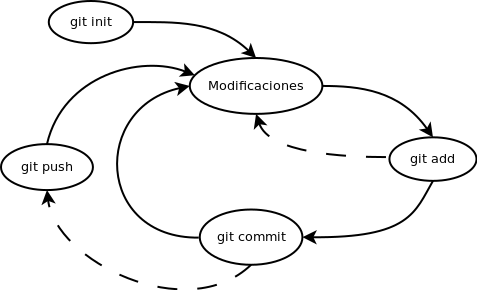
\includegraphics[height=6cm]{gitcycle.png}
\end{center}
\end{frame}

\begin{frame}
\frametitle{.gitignore}
\begin{itemize}
    \item Archivo especial en formato \emph{glob}\cite{Gitignore}.
    \item Permite mantener el repositorio minimalista al ignorar archivos generados automaticamete.
    \item Ejemplos de archivos ignorados: Codigo de maquina (*.dll).
    \item Este repositorio contiene un archivo \emph{.gitignore} en su carpeta base.
\end{itemize}
\end{frame}

\begin{frame}
\bibliography{../../Referencias/referencias}
\bibliographystyle{plain}
\end{frame}

\end{document}